\documentclass[fleqn, 10pt]{extarticle}
\usepackage{textbook}
\usepackage{placeins}
\usepackage{alltt}
%\input{vc.tex}

\begin{document}
\selectlanguage{russian}

%\title{\textbf{Восходение на подснежник}\\
%\large{Отчёт о восхождении команды а/к <<Политехник>> на в. Байчечекей, 4515 м, по ледовому кулуару западной стены (м-т Ильющенко) 4б к.сл.}}
%\author{\textsc{составила Юлия Беляева}}
\begin{titlepage}
	\clearpage\thispagestyle{empty}
	\begin{center} % Right align
		
		\vfill

		{\LARGE\textbf{Восходение на подснежник}\\
			\large{Отчёт о восхождении команды а/к <<Политехник>> на вершину Байчечекей (4515 м)
			по ледовому кулуару западной стены (маршрут Ильющенко) 4Б категории сложности}} % Increase the font size of the title

		\vspace{50pt} % Some vertical space between the title and author name

		{\textsc{составила Юлия Беляева}} % Author name

		\vspace{40pt} % Some vertical space between the author block and abstract

		\begin{figure}[ht]
			\centering
			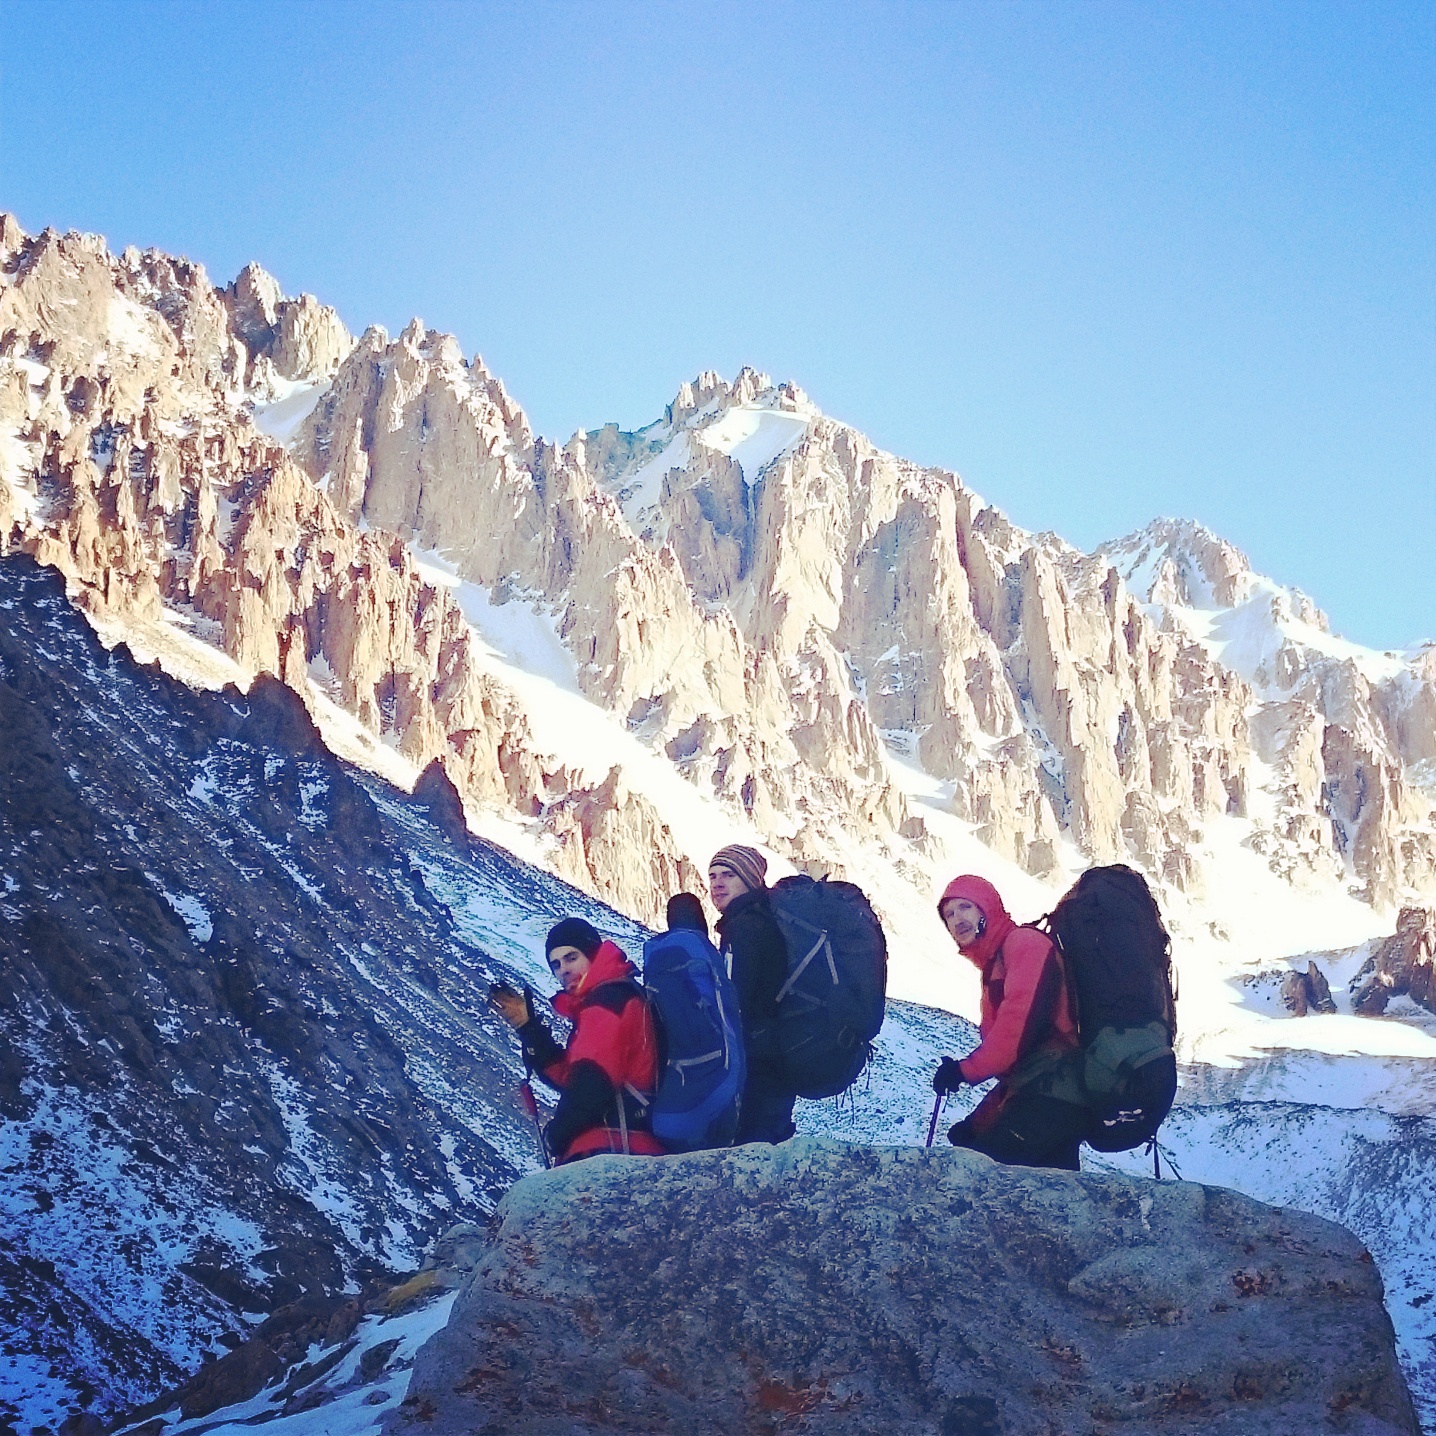
\includegraphics[width=0.7\textwidth]{title}
%			\captionof{figure}{Простейший вариант станции на дереве.}\label{fig:title}
		\end{figure}
		
		\vfill

		\today
	\end{center}
\end{titlepage}
%\maketitle

%\begin{abstract}
%	Данный отчёт составлен для участия в конкурсе отчётов а/к <<Политехник>> в 2015м году.
%\end{abstract}

\newpage\tableofcontents\newpage

\section{Обзор района}
	Район Ала-Арча находится в Кигргизском хребте в горной системе Тянь-Шань. Высота вершин около 4000-4800 метров. В районе имеется 14 ледовых и ледово-снежных маршрутов классифицированных ФАР,
	сложности от 2Б до 5Б, а также множество скальных и комбинированных маршрутов.
	
	Зимой погода в районе устойчивая, количество снега относительно небольшое. Это делает район привлекательным для зимних поездок <<за льдом>>. Базой
	может служить стоянка Рацека (3200м), где есть отапливаемая хижина и горячая еда в столовой (рис.~\ref{kotleta}). Множество маршрутов ходят прямо отсюда, для более отдалённых маршрутов есть несколько
	хижин выше.
	
	Транспортная доступность района хорошая. Для российских граждан визы в Киргизскую Республику не нужны.
	Расстояние от аэропорта города Бишкек до Национального парка Ала-Арча (2100м) составляет около 56 км (примерно час езды на автомобиле \cite{road}). Подъём на стоянки Рацека занимает до трёх часов.

	Имеется гайдбук по району~\cite{risk}, также доступны для скачивания описания на сайте ФАР (только для членов).
	\begin{figure}[h]
		\centering
		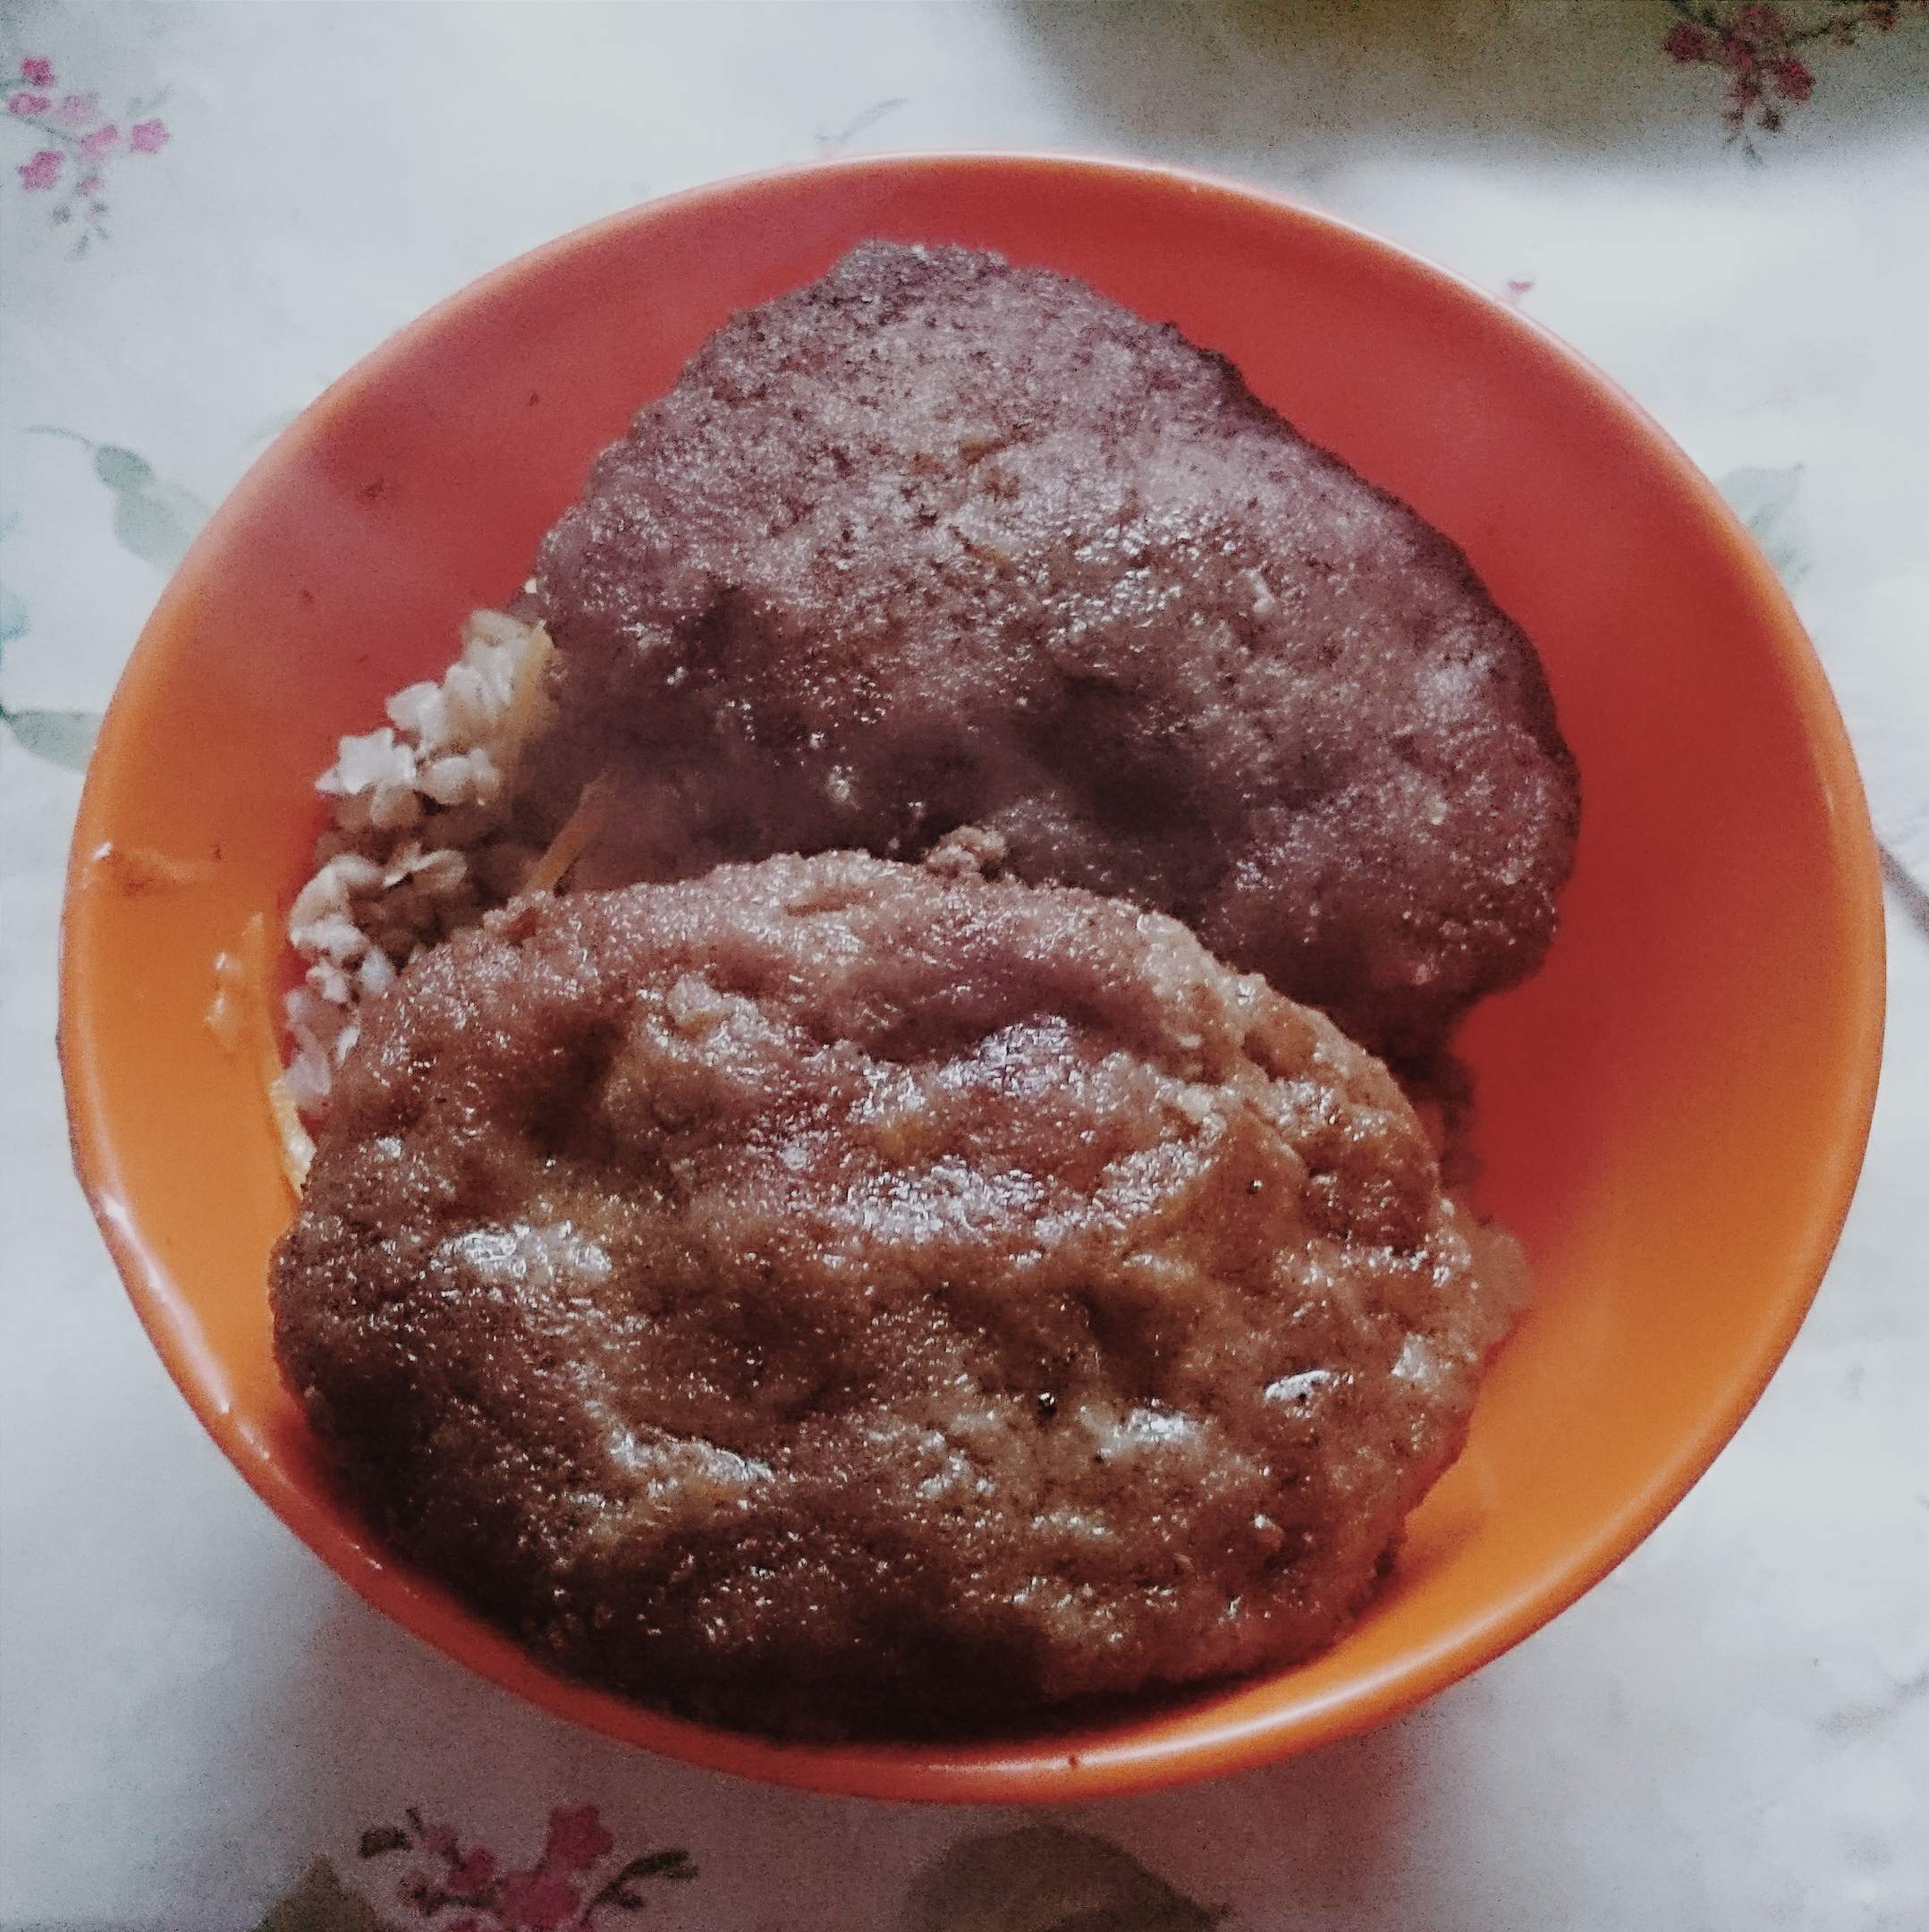
\includegraphics[width=0.7\textwidth]{kotleta}
		\caption{Две котлеты на второе в столовой Ак-Сая на стоянке Рацека.}\label{kotleta}
	\end{figure}
	\begin{figure}[H]
		\centering
		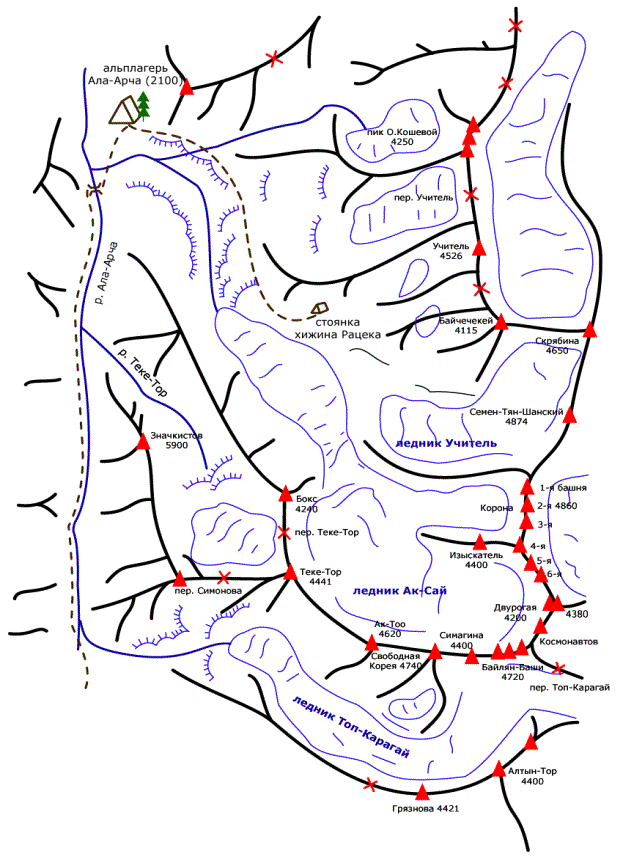
\includegraphics[width=\textwidth]{area}
		\caption{Схема района Ала-Арча \cite{uvk}.}\label{area}
	\end{figure}
\FloatBarrier
\section{Описание маршрута}
	Вид на вершину Байчечекей открывается уже с тропы на стоянки Рацека. Вертикальная линия ледового кулуара раскрывающаяся в бело-голубое ледовое поле как цветок (отсюда, по предположению автора, происходит
	название вершины: <<байчечекей>> в переводе с киргизского означает <<подснежник>>) сразу привлекает к себе внимание. По этой линии проходит маршрут по ледовому кулуару западной стены
	Ильющенко 4Б. Левее расположен ещё один ледово-снежный маршрут -- маршрут по центру северного ледового поля Селиверстова 4А. Правее, по контрфорсам западной стены, проходит несколько линий
	пятой категории сложности.
	\begin{figure}[h]
		\centering
		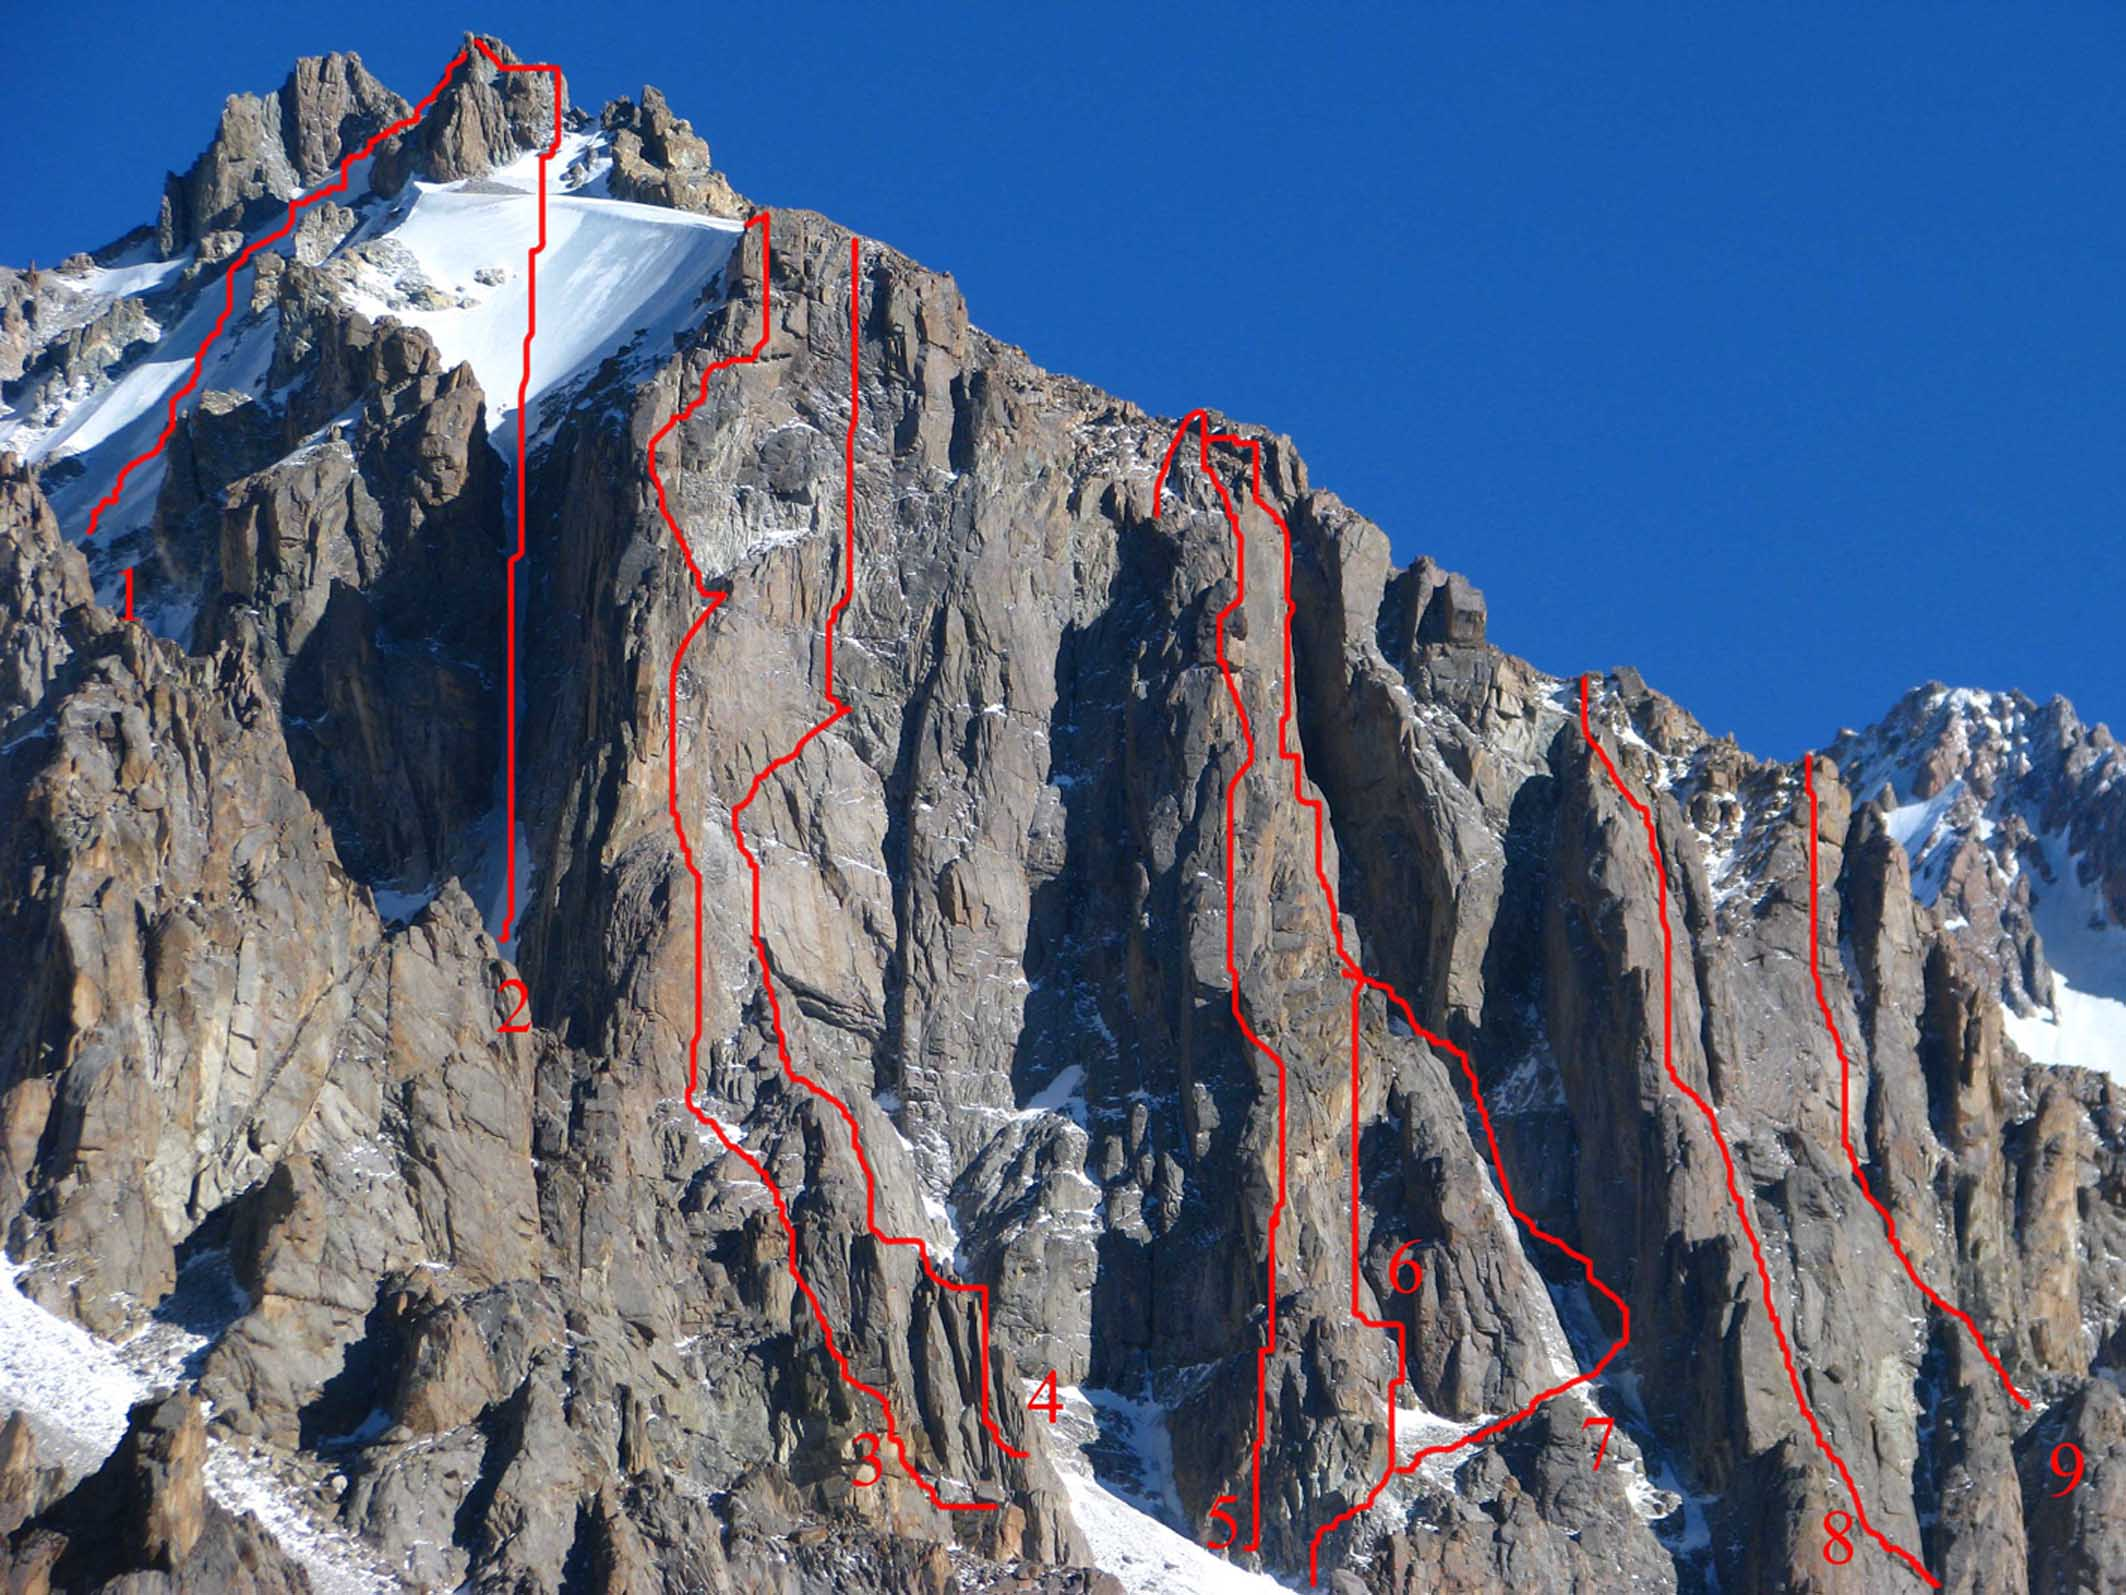
\includegraphics[width=\textwidth]{topo}
		\captionsetup{singlelinecheck=off}
		\caption[Маршруты на вершину Байчечекей]{Маршруты на вершину Байчечекей~\cite{grekov_all}:
			\begin{enumerate}
				\item С. Селиверстов 4А;
				\item А. Ильющенко 4Б;
				\item Б. Кузьменко 5А;
				\item С. Дашкевич 5А;
				\item Д. Павленко 5А;
				\item В. Поляк 5А;
				\item А. Калашников 5А;
				\item А. Шваб 5А;
				\item М. Михайлов 5А.
			\end{enumerate}}
	\end{figure}
\subsection{Общие сведения}
		\begin{tabular}{l l}
			горная система & Тянь-Шань \\
			район & Киргизский Хребет \\
			вершина & Байчечекей \\
			высота & 4515м \\
			название маршрута & по ледовому кулуару западной стены \\
			неформальное название & Сопля \\
			характер маршрута & ледово-снежный \\
			первопрохождение & А Ильюшенко, 1989 г. \\
			количество участков & 9 \\
			максимальная крутизна & $85^o$ \\
		\end{tabular}
\subsection{Подход под маршрут и спуск с маршрута}
	Подход под маршрут начинается по тропе, идущей от стоянок Рацека в сторону хижины Наука. Далее подъём идёт по осыпи под северными склонами вершины, к началу широкого некрутого
	снежно-фирнового кулара. Из этого кулуара также начинается маршрут Селиверстова 4А по центру северного ледового склона. Перед началом кулуара слева перед скальными выступами есть небольшая площадка.
	На этой площадке рекомендуется надеть кошки и обвязки, так как в кулуаре удобного места не будет. Подъём продолжается по кулуару до начала маршрута (рис.~\ref{start}).

	Спуск с маршрута проходит по осыпному кулуару засыпанному снегом (рис. ~\ref{descend}) на южной стороне вершины, смотрящему на пик Семёнова-Тян-Шанского, вниз до ледника Учитель.
	От окончания маршрута до спускового кулуара можно
	добраться траверсом склона вокруг вершинной башни против часовой стрелки. Важно попасть в нужный кулуар: если начать спуск раньше то можно выйти на сбросы. В январе осыпь покрыта тонким слоем
	снега с плотной коркой которая проламывается под ногами спускающихся. После спуска на ледник, надо продолжить движение вдоль него, огибая южные и западные
	склоны горы двигаясь в сторону подъёмной тропы. Аварийный спуск возможен дюльферами по пути подъёма.
	\begin{figure}[ht]
		\centering
		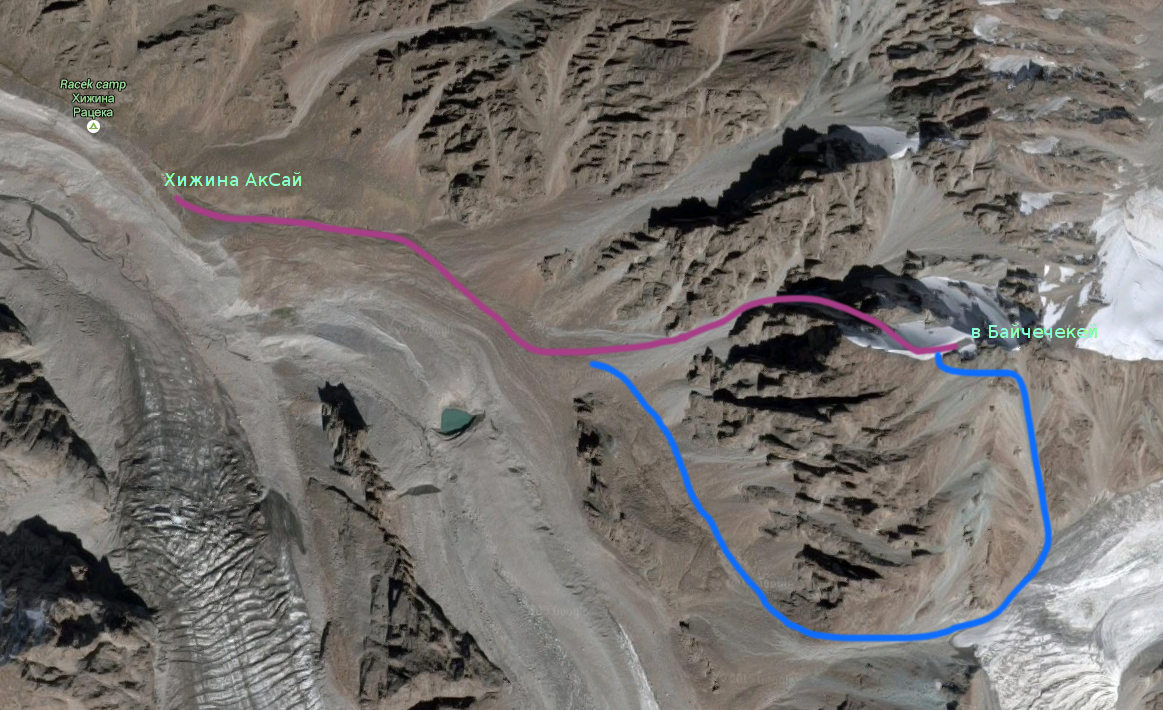
\includegraphics[width=\textwidth]{map}
		\caption{Маршрут на снимке из космоса. Розовым цветом показан путь подъёма, синим -- спуска.}
	\end{figure}
	\begin{figure}[ht]
		\centering
		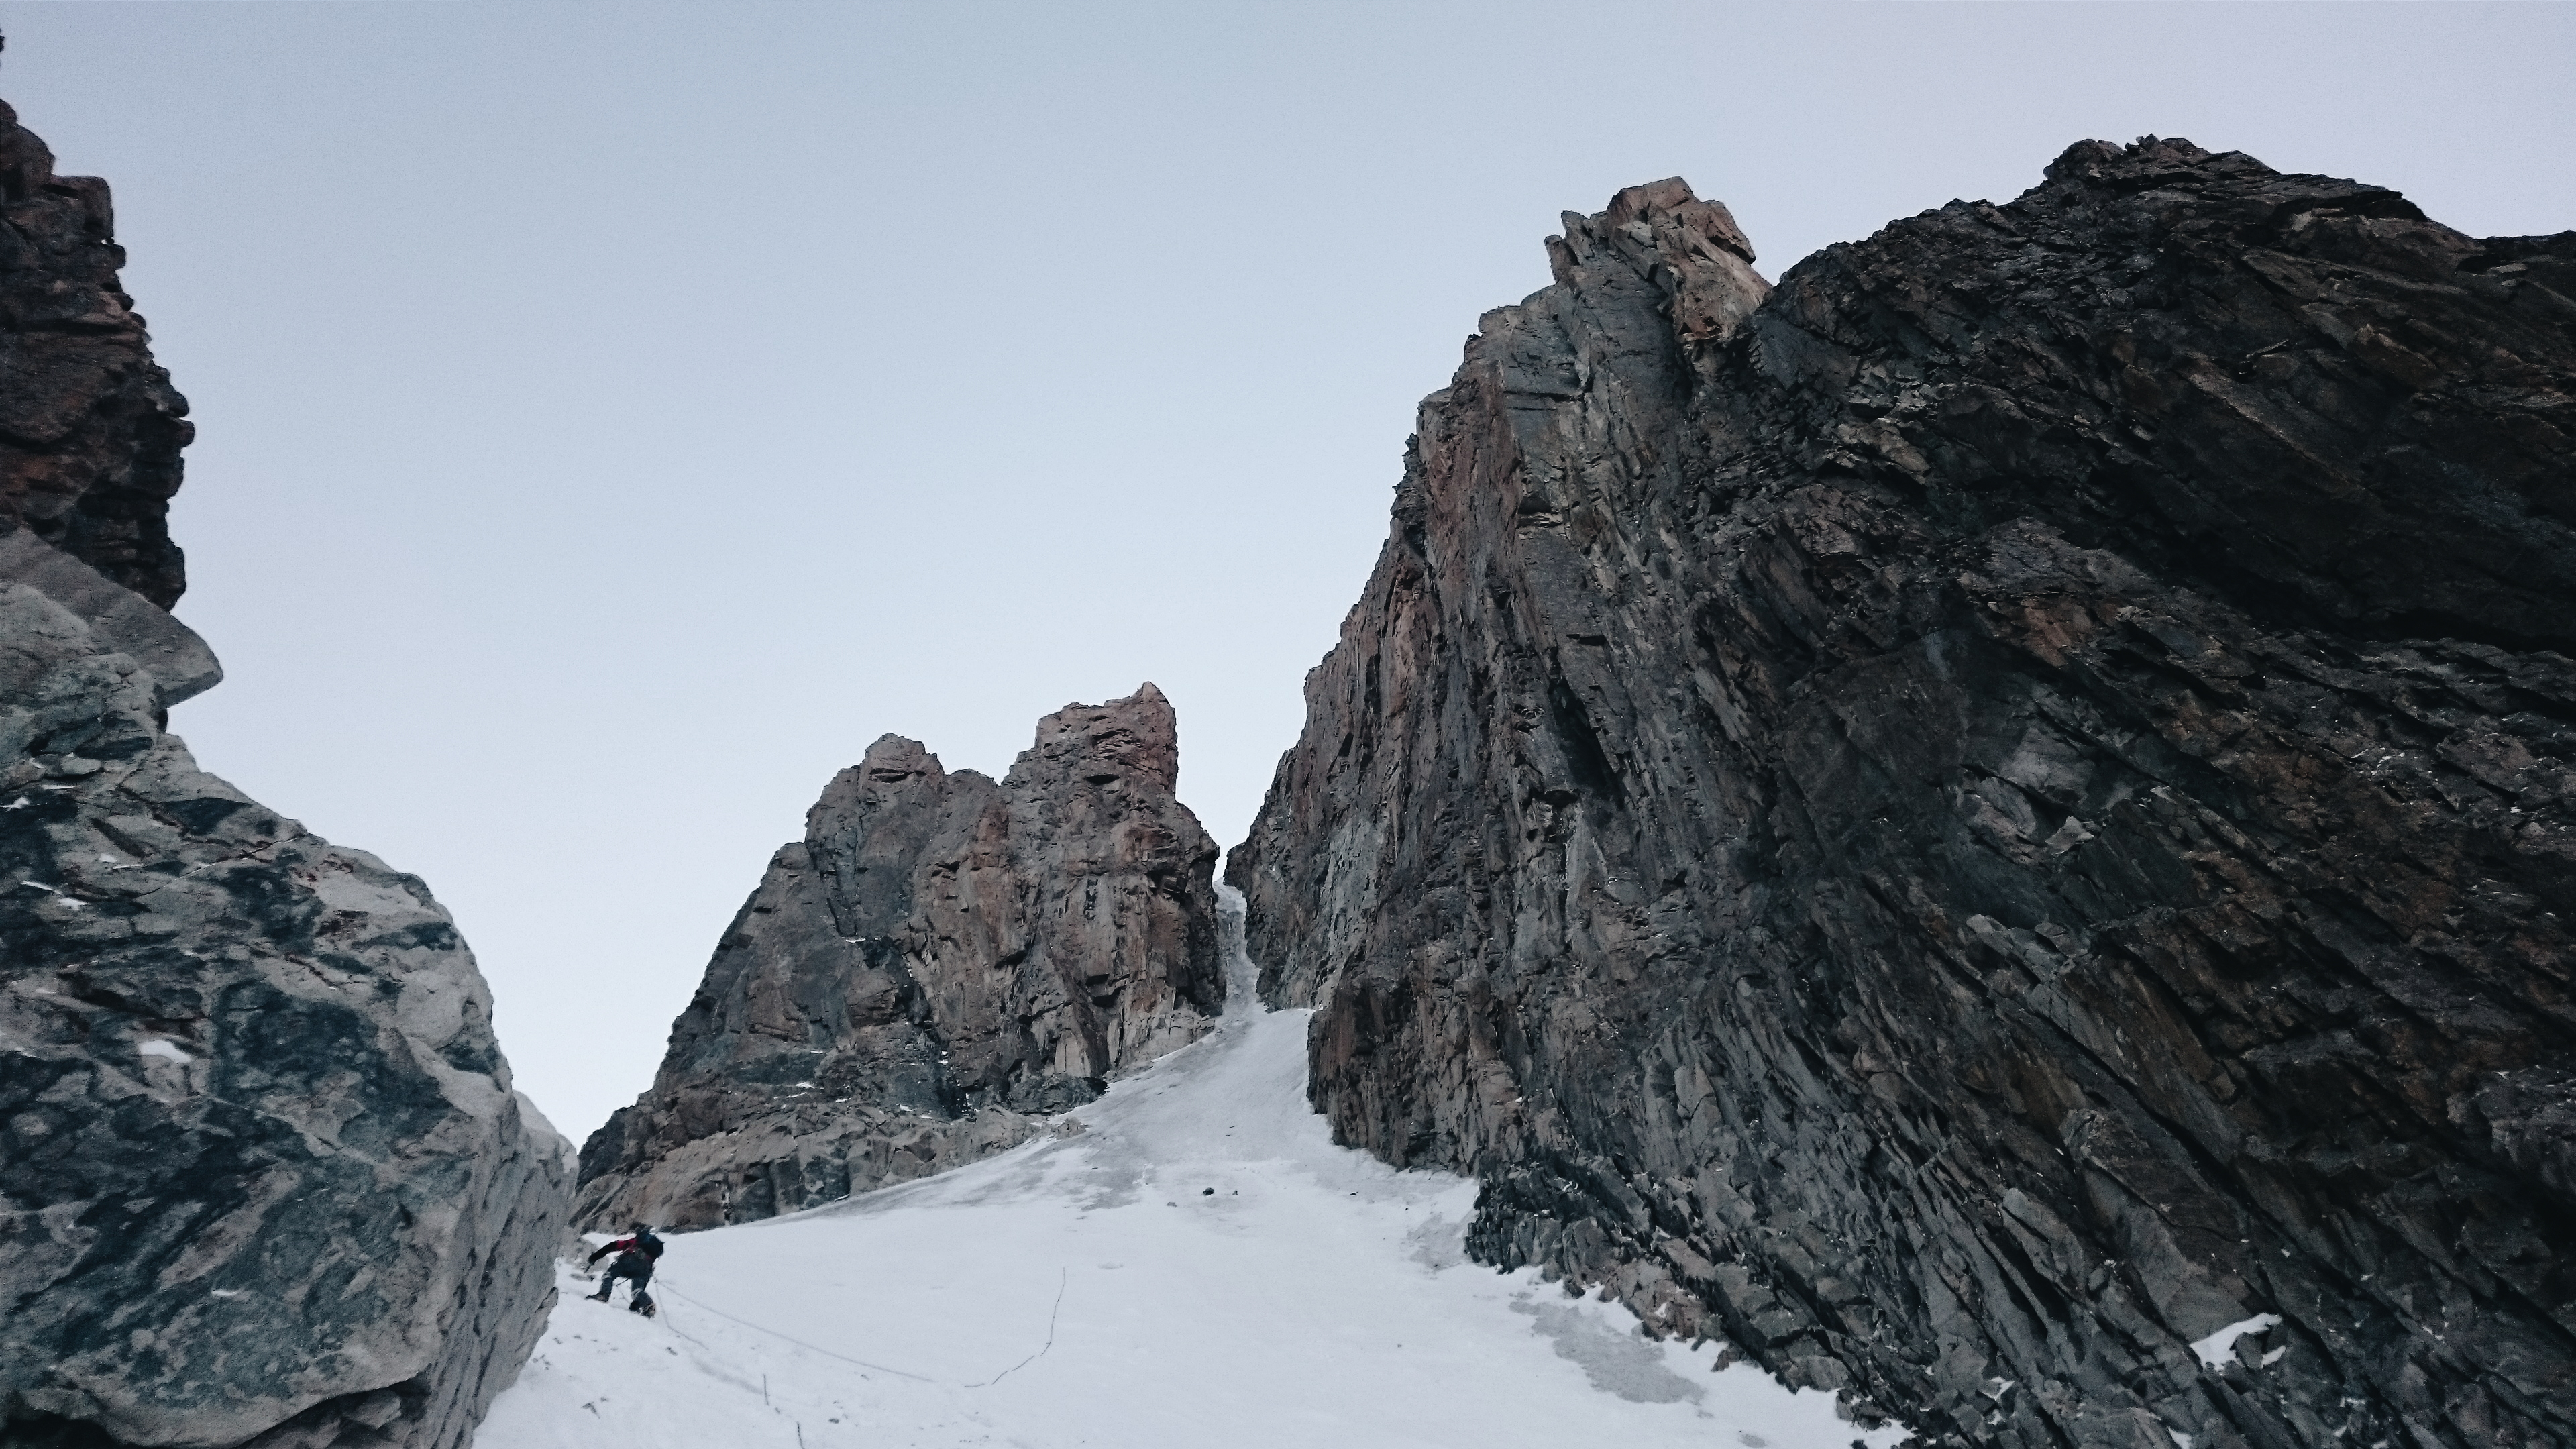
\includegraphics[width=\textwidth]{upview}
		\caption{Вид на начало маршрута.}\label{start}
	\end{figure}\begin{figure}[ht]
		\centering
		\includegraphics[width=\textwidth]{descend}
		\caption{Спусковой кулар. Фото сделано на маршруте Селиверстова, траверс склона от маршрута Ильющенко выводит ниже по этому кулуару.}\label{descend}
	\end{figure}
\FloatBarrier
\subsection{Схема и фотографии участков маршрута}
	\begin{figure}[ht]
		\centering
		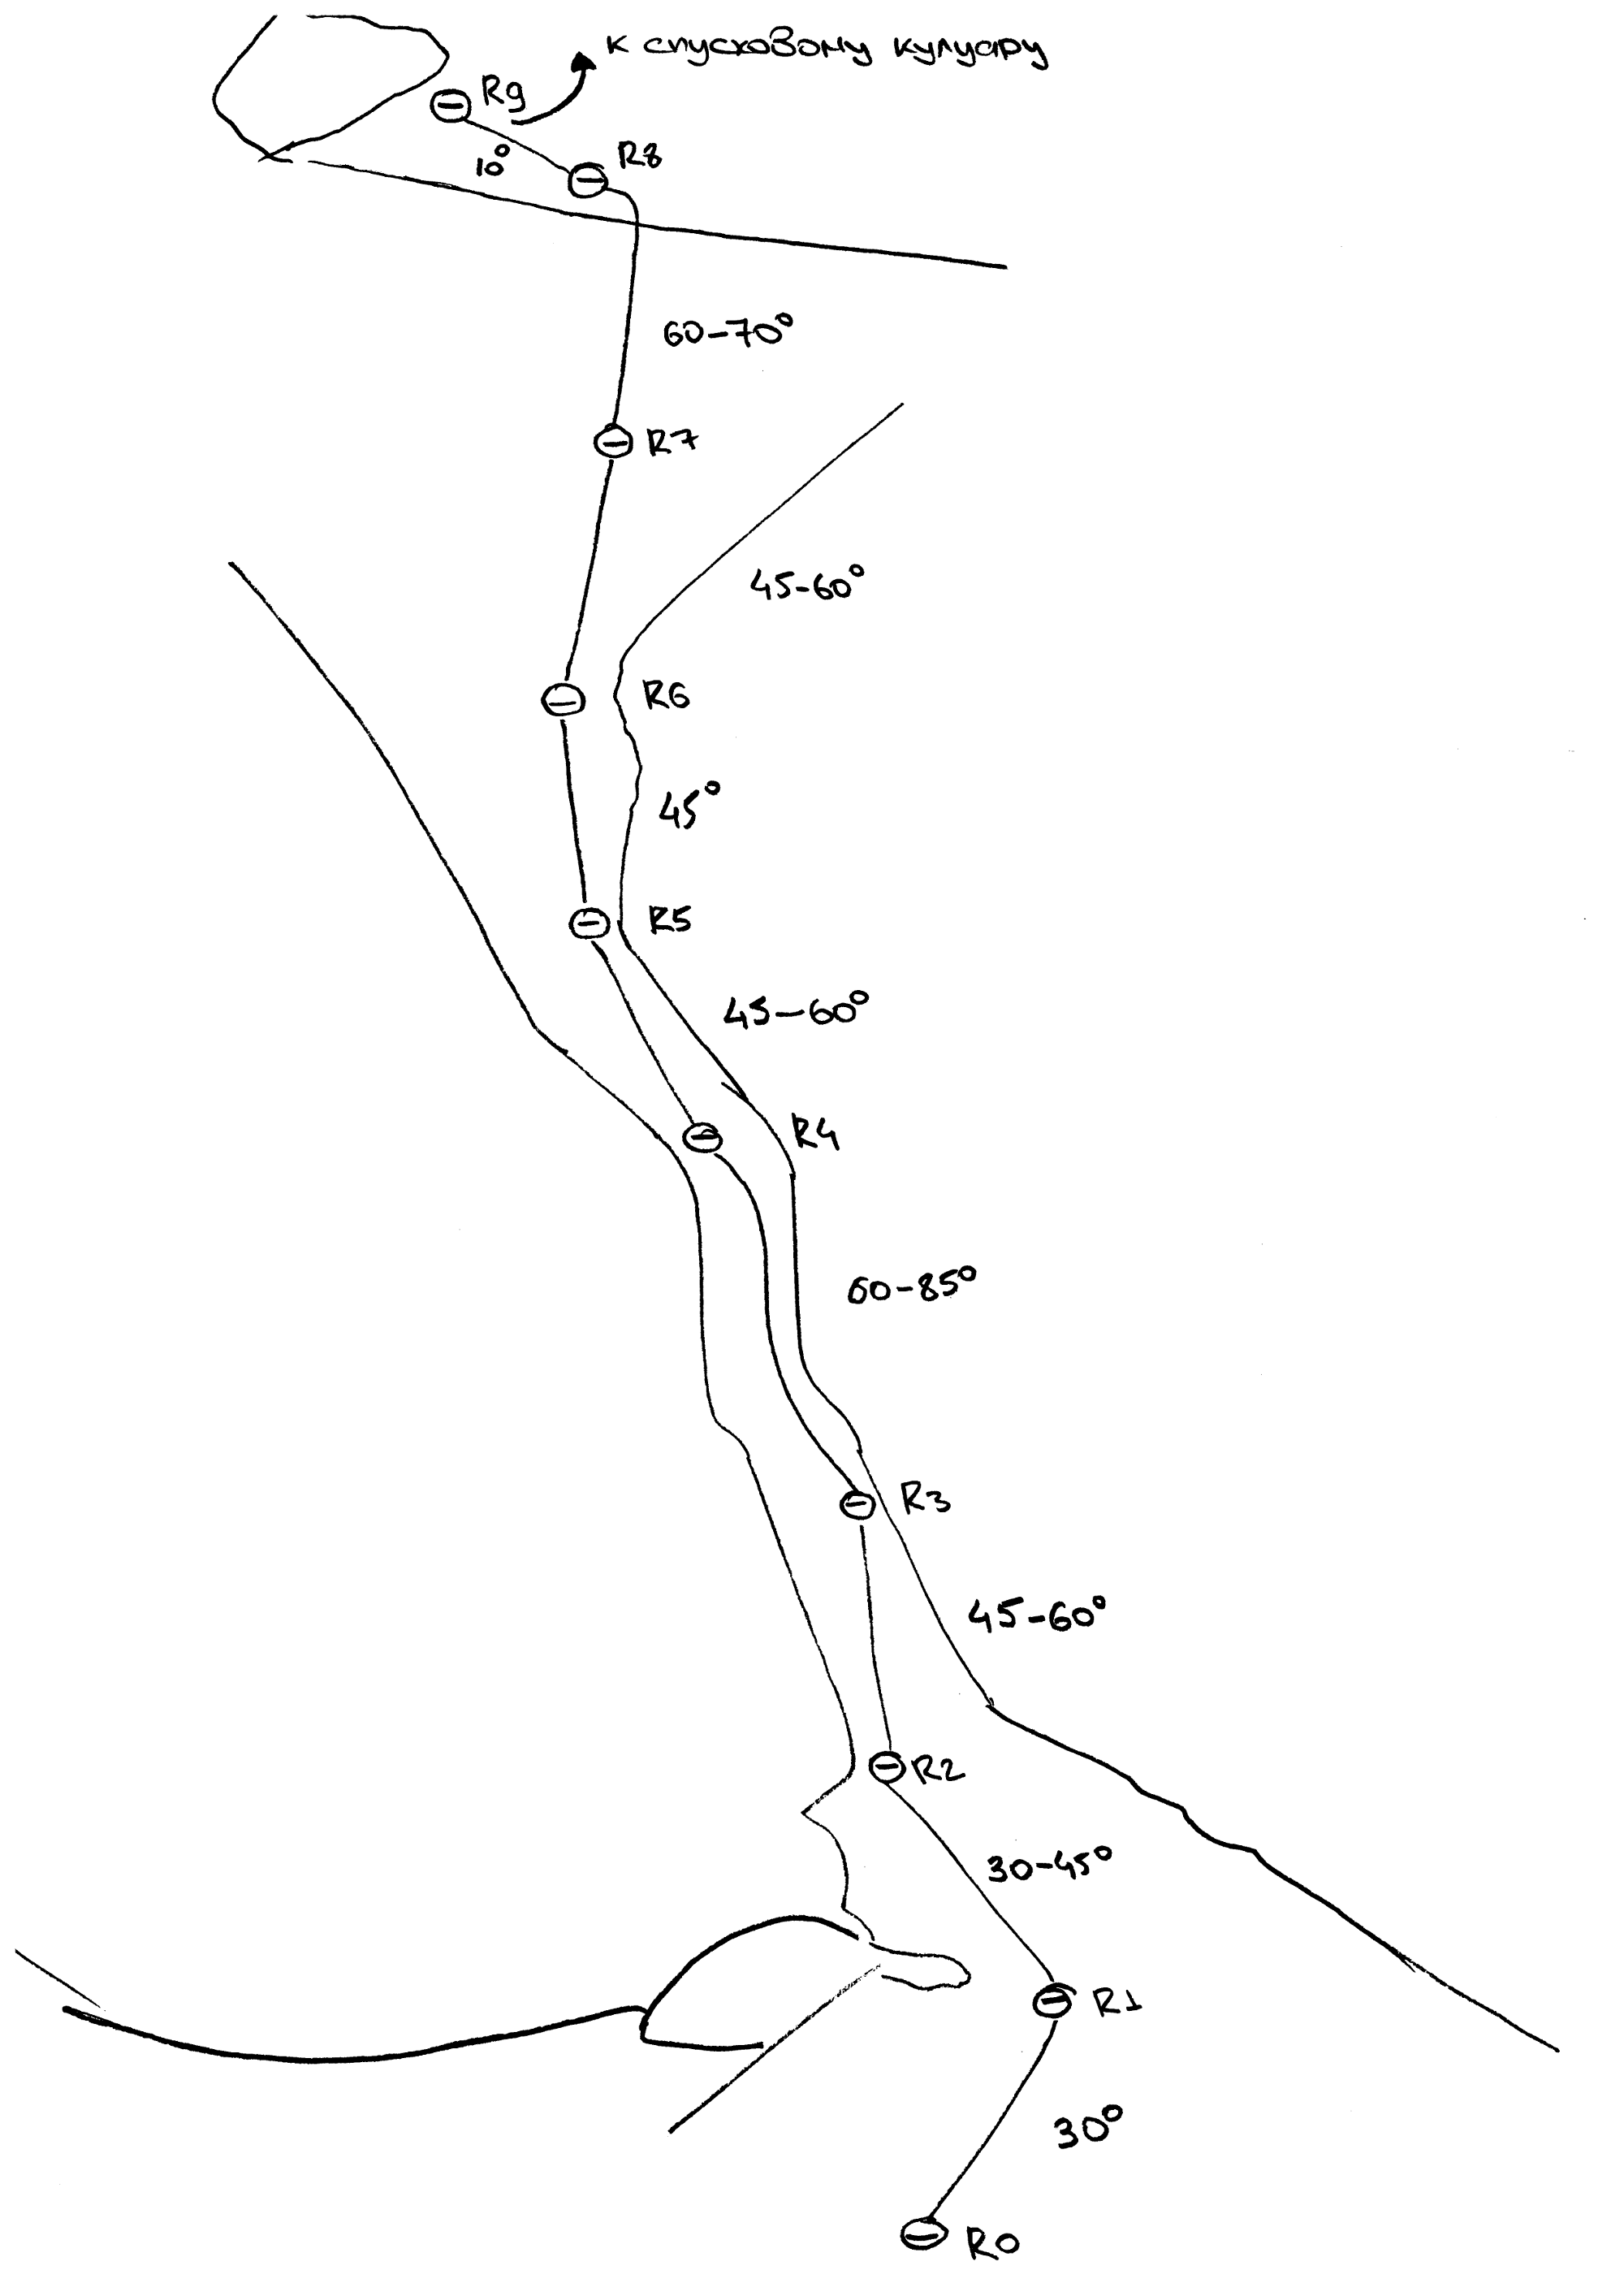
\includegraphics[width=0.8\textwidth]{uiaa}
		\caption{Схема маршрута. Расстояние между станциями ~50м. Подписанные значения крутизны участков очень условны.}\label{uiaa}
	\end{figure}
	\begin{figure}[ht]
		\centering
		\includegraphics[width=\textwidth]{r1r2}
		\caption{Участки R1 и R2 -- подлаз.}\label{r1r2}
	\end{figure}
	\begin{figure}[ht]
		\centering
		\includegraphics[width=\textwidth]{r3}
		\caption{Участок R3 -- предвкушение ключа.}\label{r3}
	\end{figure}
	\begin{figure}[ht]
		\centering
		\includegraphics[width=\textwidth]{r4}
		\caption{Участок R4 -- ключ маршрута.}\label{r4}
	\end{figure}
	\begin{figure}[ht]
		\centering
		\includegraphics[width=\textwidth]{r5}
		\caption{Участок R5 -- здесь ещё кажется что финал близок.}\label{r5}
	\end{figure}
	\begin{figure}[ht]
		\centering
		\includegraphics[width=\textwidth]{r6}
		\caption{Участок R6 -- подозрения о том, что финал не близок.}\label{r6}
	\end{figure}
	\begin{figure}[ht]
		\centering
		\includegraphics[width=\textwidth]{r7}
		\caption{Участок R7 -- выход из <<стебелька>>.}\label{r1r2}
	\end{figure}
	\begin{figure}[ht]
		\centering
		\includegraphics[width=\textwidth]{r8}
		\caption{Участок R8 -- лёд прекрасен.}\label{r8}
	\end{figure}
	\begin{figure}[ht]
		\centering
		\includegraphics[width=\textwidth]{r9}
		\caption{Участок R9 -- можно успеть к ужину.}\label{r9}
	\end{figure}
	\FloatBarrier

\subsection{Безопасность}
	В феврале 2015го года на этом маршруте произошло ЧП с членом альпклуба Политехник Фёдором Гуторовым, который получил тяжёлую ЧМТ. Важно помнить,
	что маршрут не является полностью безопасным,
	а усталость после прохождения ключа может снизить концентрацию лидера и привести к ошибкам.
	
	В зимнее время основной опасностью на маршруте может оказаться лёд плохого качества (с пустотами или выкалывающийся линзами).
	Это прежде всего относится к участкам в кулуаре, в особенности на ключе. Меры предосторожности -- внимательность лидера при лазаньи и закручивании буров, осмотр участка льда
	и зачистка верхнего слоя при необходимости. Вторая возможная опасность -- удар о скальные стенки кулуара при срыве. Поэтому нужно стараться избегать возможного маятника при падении, внимательно выбирая линию
	движения по кулуару и устанавливая точки страховки в нужных местах.
	Также следует с осторожностью относиться вмёрзшим в лёд старым проушинам и если и использовать их для страховки, то только в качестве дополнительных точек.

\section{Информация о восхождении}
	Восхождение по маршруту было совершено 6го января 2015го года командой альпклуба Политехник в составе: Ильин Евгений (руководитель, 2 с.р.), Коваленко Дмитрий (2 с.р.),
	Лаевский Игорь (первый на маршруте, 2 с.р.), Беляева Юлия (автор отчёта, 2 с.р.). Для подготовки к восхождению были проведены занятия на леднике Ак-Сай для
	тренировки лазанья по льду, работы в связках, организации станций и ледовых проушин. Также были совершены акклиматизационное восхождение на вершину Учитель по западному гребню (1Б) 
	и тренировочные ледовые восхождения вершину
	Корона (2-я) по правому кулуару С стены (3Б) Акимова и Байчечекей по центру С ледового склона (4А) Селиверстова. На восхождении по маршруту Селиверстова было просмотрено начало маршрута
	(рис.~\ref{start}), а так же спусковой кулуар (рис.~\ref{descend}). К сожалению, от начала маршрута не видно верхних верёвок и в целом начало кажется короче чем оно есть на самом деле.
	Перед восхождением были получены консультации по маршруту у инструкторов.

	Схема работы в четвёрке была избрана следующая: первый лезет с двумя верёвками, прощёлкивая одну из них в точки страховки и вытягивая вторую. Организовав станцию, принимает одновременно
	второго и третьего. Третий участник вытягивает верёвку четвёртого. Затем второй выпускает первого на следующий участок, а третий принимает последнего. Перила во время восхождения не применялись.

	Все участники кроме автора использовали для лазанья ледовые фифы. Не смотря на то, что фифы позволяют преодолевать ледовые склоны с большой скоростью, автору нравится пользоваться
	инструментами так как это гораздо веселее (и мышцы в процессе можно накачать). На пологих участках можно экономить силы идя на ногах, при этом просто опираясь на инструменты
	держа их руками под головкой, не забивая, а втыкая клювик в лёд. Но на крутых участках, конечно, надо бить (и в этом раскрывается вся суть инструментов). Бить было здорово.
	В особенности здорово было на ключе маршрута. Ключ оказался не ровным, а бугристым, имеющим рельеф. Инструмент заходил в такой лёд хорошо, а рельеф помогал ставить ноги. В целом лазанье
	было приятным, хотя конечно к последним верёвкам накопилась усталость.

	Прохождение маршрута заняло 8 часов, 12 часов с учётом подхода и спуска.

\section{Заключение}
	Маршрут Ильющенко по ледовому кулуару западной стены на вершину Байчечекей красив и интересен.
	Рекомендуется к прохождению.

\newpage
\nocite{*}
\bibliographystyle{plain}
\bibliography{archa}
\end{document}
